\section{Quantum GIS 1.0.0}
\pagenumbering{arabic}
\setcounter{page}{1}

Quantum GIS (QGIS) is a cross-platform (GNU/Linux, MS Windows, Mac OSX) open
source application with a growing number of common GIS features and
functions. QGIS is licensed under the GNU General Public License and an
official member project of the Open Source Geospatial Foundation (OSGeo). The
current official version is 1.0.0, aka "Kore" and was released on January 05,
2009. 

\subsection{History}

The idea for Quantum GIS was born in the beginning of 2002 when Gary Sherman
began looking for a GIS viewer for Linux that was fast and supported a wide
range of data stores. That, coupled with an interest in coding a GIS
application led to the creation of the project. In the beginning Quantum GIS
was established as a project on SourceForge in June 2002 with the first,
mostly non-functioning release on July 19, 2002. This first release supported
only PostGIS layers.

Within the last 7 years, the project 

\subsection{QGIS Community}

\begin{figure}[h]
   \begin{center}
   \caption{QGIS Community Map}\label{fig:community-map}\smallskip
   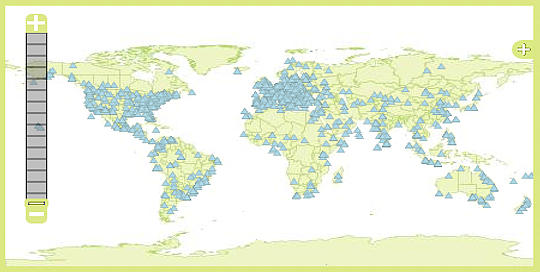
\includegraphics[clip=true]{community-map}
\end{center}
\end{figure}

\subsection{Functionality}



\subsection{Development}

\subsection{Conclusion}

\minisec{Authors}

The authors of this article are QGIS Project Steering Committee Members:

Otto Dassau <dassau@nature-consult.de>  
\\Gary Sherman <sherman@mrcc.com>
\\Tim Sutton <tim@linfinity.com>
\\Marco Hugentobler <marco.hugentobler@karto.baug.ethz.ch>
\\Paolo Cavallini <cavallini@faunalia.it>

\minisec{Links}

For more information, have a look at the following website:

Quantum GIS website: http://qgis.osgeo.org



 



